\documentclass[10pt,twocolumn,letterpaper]{article}

\usepackage{cvpr}
\usepackage{times}
\usepackage{epsfig}
\usepackage{graphicx}
\usepackage{amsmath}
\usepackage{amssymb}
\usepackage{listings}
\usepackage{algorithm}
\usepackage[noend]{algpseudocode}
\usepackage{fancyvrb}
\usepackage{xcolor}

\usepackage{url}


\setcounter{secnumdepth}{4}
% New Line after Paragraph
\newcommand{\nlparagraph}[1]{\paragraph{#1}\mbox{}\\}

\cvprfinalcopy % *** Uncomment this line for the final submission

\def\cvprPaperID{****} % *** Enter the CVPR Paper ID here
\def\httilde{\mbox{\tt\raisebox{-.5ex}{\symbol{126}}}}

\makeatletter
\def\BState{\State\hskip-\ALG@thistlm}
\makeatother

% Algorithm Script Size
\makeatletter
\algrenewcommand\ALG@beginalgorithmic{\scriptsize}
\makeatother

% Needed to show code snippets...
\DefineVerbatimEnvironment{Highlighting}{Verbatim}{commandchars=\\\{\}}
\newenvironment{Shaded}{}{}
\newcommand{\StringTok}[1]{\textcolor[rgb]{0.25,0.44,0.63}{#1}}
\newcommand{\AttributeTok}[1]{\textcolor[rgb]{0.49,0.56,0.16}{#1}}
\newcommand{\ExtensionTok}[1]{#1}
\newcommand{\NormalTok}[1]{#1}
\lstdefinestyle{CSnippetStyle}{
  language=C,
  numbers=left,
  stepnumber=1,
  numbersep=10pt,
  tabsize=2,
  breaklines=true,
  showspaces=false,
  numbersep=5pt,
  showstringspaces=false,
  captionpos=b,
  % Colors and Font
  basicstyle=\footnotesize\ttfamily,
  keywordstyle=\bfseries\color{green!40!black},
  commentstyle=\itshape\color{purple!40!black},
  identifierstyle=\color{blue},
  stringstyle=\color{orange},
}

\graphicspath{ {./images/} }



% Pages are numbered in submission mode, and unnumbered in camera-ready
\ifcvprfinal\pagestyle{empty}\fi
\begin{document}

%%%%%%%%% TITLE
\title{K-Means Clustering Algorithm}

\author{Adriano Di Dio\\
E-mail address\\
{\tt\small adriano.didio@stud.unifi.it}
}

\maketitle
\thispagestyle{empty}

%%%%%%%%% ABSTRACT
\begin{abstract}
Purpose of this paper is to describe how the K-Means Clustering Algorithm works and how it can be implemented using a 
programming language.\newline
In particular, it will be shown how to implement the main algorithm in C and how it can be sped up using multiple threads through the 
CUDA framework.
\end{abstract}

%%%%%%%%% BODY TEXT
\noindent\large\textbf{Future Distribution Permission}\\
\indent The author(s) of this report give permission for this document to be distributed to Unifi-affiliated students taking future courses.

\section{Introduction}
K-Means Clustering is an algorithm which is used to partition a set of points into k clusters in which each point belongs to the cluster
with the smaller distance from the center that is called centroid.\newline
The main algorithm can be divided into 4 main steps:
\begin{itemize}
  \item Initialization Phase
  \item Assignment Step.
  \item Update Step.
  \item Convergence Check Step.
\end{itemize}
Details about each one will be given in the next chapters, in particular in chapter 2 a brief explanation of the algorithm is 
given and a sample implementation using pseudo-code is shown, then in chapter 3 and 4 the sequential and parallel version is 
described, and finally, in the last chapter, the performance will be evaluated by showing the differences between the 
sequential and parallel version.\newline

\vspace{3cm}

%-------------------------------------------------------------------------
\section{Algorithm}

K-Means algorithm, as stated in the introduction, is made of four steps that alternates until the last one, that represents 
the exit condition, tells the algorithm to stop since there are no updates to the centroids position.\newline
In order to describe it we need to define a few key elements.\newline
First we need to define the data-set as a group of d-dimensional points:\newline

\begin{equation} 
\label{eq:Data-Set}
(x\textsubscript{1},x\textsubscript{2},x\textsubscript{3},\cdots,x\textsubscript{n})
\end{equation}

Then we need to define our centroids as a set made of k elements ($k \leq n$):\newline
\begin{equation} 
\label{eq:Data-Set}
S=\{S\textsubscript{1},S\textsubscript{2},S\textsubscript{3},\cdots,S\textsubscript{k}\}
\end{equation}
the goal is to partition the data-set into k clusters to minimize the within-cluster distance between each point and the centroids.
\newline
The first step is the Initialization Phase, in this phase, the algorithm has to find some random points that will be used as 
centroids to initialize it.\newline
In this implementation the initial centroids are chosen from the starting k points contained in the data-set, this enable the 
algorithm to be predictable so that the differences between sequential and parallel version won't depends from the centroid's 
starting position,as long as the data-set is kept the same.
\newline
Then the clusters are calculated using the chosen centroid's position, by calculating the distance between each point and 
centroid, that are then assigned to the nearest centroid:\newline
\begin{multline}
\label{eq:Centroids}
S_i^{(t)} =\\
\left \{ x_p : \left \| x_p - m^{(t)}_i \right \|^2 \le \left \| x_p - m^{(t)}_j \right \|^2 \ \forall j, 1 \le j \le k \right\}\\
\end{multline}

since we now have created a new cluster made of n-points the centroid's position needs to be updated by calculating the new 
mean value based on the position of all the points inside the cluster:\newline
\begin{equation}
\label{eq:first}
m^{(t+1)}_i = \frac{1}{\left|S^{(t)}_i\right|} \sum_{x_j \in S^{(t)}_i} x_j 
\end{equation}  

The algorithm, repeats these two steps until the updated centroid's position is not so much different from the old centroid's 
position, in fact, if the distance between the new cluster position and the old one is negligible then the algorithm is said to 
have converged and the algorithm stops.
\\
Below, a pseudo-code implementation of the algorithm:\\
\subsection{Pseudo-Code}
An example implementation can be seen below:
\begin{algorithm}
\caption{KMeansAlgorithm\newline
Takes 3 parameters:Dataset,Number Of Points,Number of Centroids}\label{euclid}
\begin{algorithmic}[1]
\Procedure{KMeansAlgorithm}{Dataset[],n,k}
	\For{\texttt{$i \gets 1$ to $k$}}
        \State \texttt{Centroid[i] = Dataset[i]}
    \EndFor
    \While{true}
       	\State {$SetClusters$ $\gets$ {0}}
    		\For{\texttt{$i \gets 1$ to $n$}}
    		    \State {$Min$ $\gets$ {-INF}}
    			\For{\texttt{$j \gets 1$ to $k$}}
        			\State {$Dist$ $\gets$ {$Dist(Dataset_{i},Centroid_{j})$}}
        			\If {$Dist < Min$}
        				\State {$Min$ $\gets$ {$Dist$}}
        				\State {$Cluster_{i}$ $\gets$ {$Centroid_j$}}
        			\EndIf
    			\EndFor
    		\EndFor
    		\For{\texttt{$i \gets 1$ to $k$}}
    		    \State {$ClusterSize$ $\gets$ {0}}
    		    \State {$Sum$ $\gets$ {0}}
    			\For{\texttt{$j \gets 1$ to $n$}}
        			\If {$Cluster_{i} \neq i$}
    					\State \textbf{continue}
        			\EndIf
        			\State {$Sum$ $\gets$ {$Sum + Dataset_{j}$}}
				\State {$ClusterSize$ $\gets$ {$ClusterSize + 1$}}
    			\EndFor
    			\State {$Sum$ $\gets$ {$Sum / ClusterSize$}}
			\State {$Delta$ $\gets$ {$VSub(Sum,Centroids_{i})$}}
			\If {$Delta>Threshold$}
    				\State \textbf{continue}
        		\EndIf
        		\State {$SetClusters$ $\gets$ {$SetCluster + 1$}}
    		\EndFor
    		\If {$SetClusters == k$}
    			\State \textbf{exit}
        	\EndIf
    \EndWhile
\EndProcedure
\end{algorithmic}
\end{algorithm}
\newpage


\section{Implementation}
\subsection{Tools}
Tools are used to generate the data-set and to plot the result of the algorithm.\newline
They works only in 2D and are able to load/save only using the csv\footnote{Comma-Separated-Value} file format and works only
using python 3.
\subsubsection{BlobGenerator}
This python script is used to generate a bi dimensional data-set that is saved in a csv file.\newline
\subsubsection{Usage}
The usage is simple and requires just to call the script in a console:\newline
\begin{Shaded}
\begin{Highlighting}[]
\NormalTok{\$ }\ExtensionTok{python3}\NormalTok{ PyBlobGenerator.py }
\end{Highlighting}
\end{Shaded}

\begin{figure}[H]
\centering
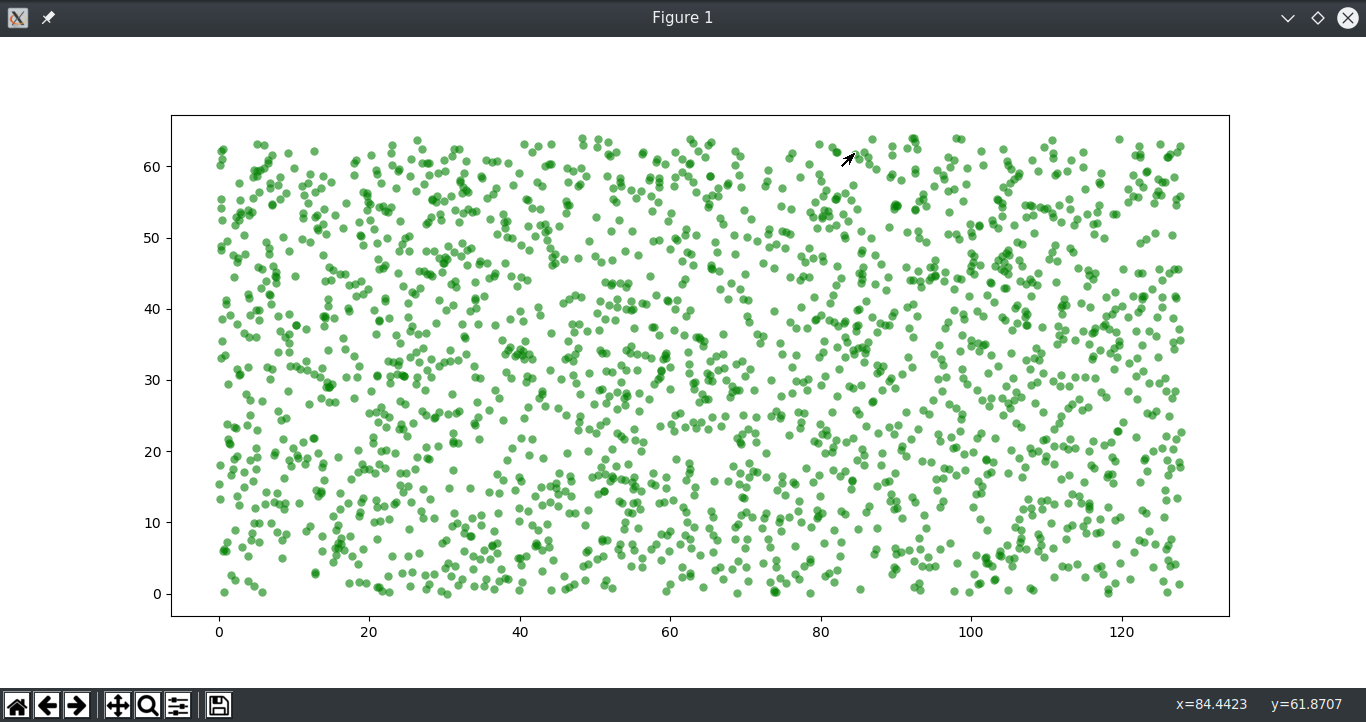
\includegraphics[width=0.3\textwidth]{Py_Blob_Generator}
\caption{PyBlobGenerator}
\end{figure}

This, by default will generate a csv file named `data\_blob.csv' containing 2048 random points.\newline
It is possible to specify the output file name:\newline

\begin{Shaded}
\begin{Highlighting}[]
\NormalTok{\$ }\ExtensionTok{python3}\\
\NormalTok{ PyBlobGenerator.py -o FileName.csv}
\end{Highlighting}
\end{Shaded}
and it can also generate an higher/lower number of points by using the parameters width and height.\newline
These two parameters defines the region in which the point must be generated.\newline
Finally it is possible to view the points in a plot by running the command:\newline
\NormalTok{\$ }\ExtensionTok{python3}\NormalTok{ PyBlobGenerator.py -s }\\
Full usage example:\newline
\NormalTok{\$ }\ExtensionTok{python3}\NormalTok{ PyBlobGenerator.py -s -o OutFile.csv -w 128 -he 128 }\newline
In this example the script will generate a random distribution of points within a 128x128 region,will save the output file in 
OutFile.csv and before saving will show a window containing the plot.\newline
\subsubsection{PlotGenerator}
This python script is used to show the result of the K-Means Algorithm by loading up to n, where n is the number of steps to view, csv 
files from the `In' folder.\newline
The main program,in facts, outputs the result as a pair of file containing the data-set and the centroids.\newline
\subsubsection{Usage}
It only takes one parameters which is the number of steps to show and will display a single windows containing up to n plots stacked
horizontally,each displaying a specific step of the algorithm:\newline
\begin{Shaded}
\begin{Highlighting}[]
\NormalTok{\$ }\ExtensionTok{python3} \NormalTok{ PyPlotGenerator.py 1}
\end{Highlighting}
\end{Shaded}

\begin{figure}[H]
\centering
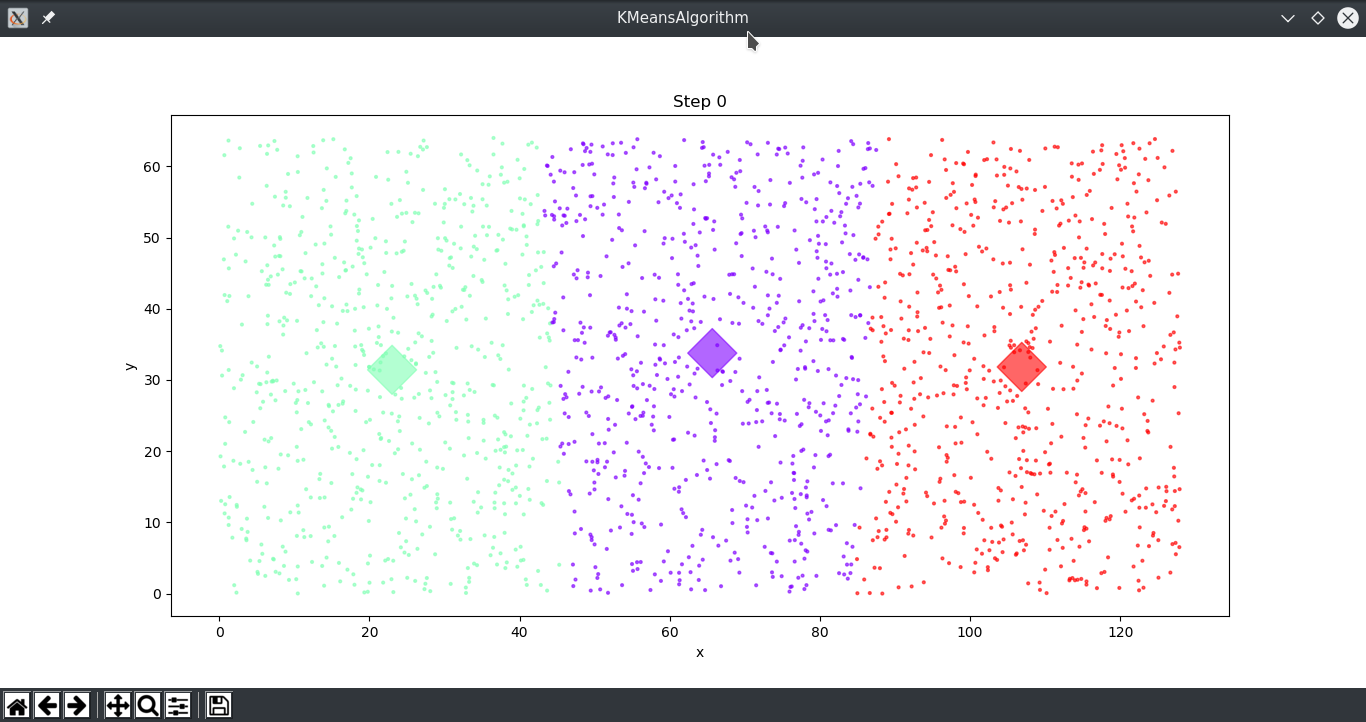
\includegraphics[width=0.3\textwidth]{Py_Plot_Generator}
\caption{PyPlotGenerator}
\end{figure}


\subsection{Main Program}
The algorithm is implemented in C and, as it can be seen from the Tools, it uses a fixed data-set that is loaded from a csv file.
\newline
This is done in order to be able to compare the sequential and parallel version, and see the difference in terms of execution 
times,without having to worry about the possible differences that can happens due to a different choice of Centroids/Points.
\newline
The program is able to read the csv file and infer the vector dimension, called `Stride' in the source code,in order to 
determine if the algorithm has to run on 2D,3D etc\ldots \newline
The program takes two arguments: the path to the dataset file in csv format and the number of centroids.\\
E.G:
\begin{Shaded}
\begin{Highlighting}[]
\NormalTok{\$ }\ExtensionTok{./KMeans} \NormalTok{ Dataset.csv 10}
\end{Highlighting}
\end{Shaded}
\subsubsection{Sequential Version}
The sequential version is made using a single function that contains an infinite loop that repeats all the required step until the exit
condition is hit.\\
The following structure have been declared to define a point and a centroid:
\begin{lstinputlisting}[language=C,style=CSnippetStyle,caption=Data Structure Definition ]{
	"codes/Sequential/KMeansClustering.h"}
\end{lstinputlisting}
The code can be divided in n parts:\\

First we need to initialize the algorithm by choosing the centroids:\\

\begin{lstinputlisting}[language=C,style=CSnippetStyle,caption=Centroids Initialization,firstline=54,lastline=61 ]{
	"codes/Sequential/KMeansClustering.c"}
\end{lstinputlisting}

As it can be seen from the snippet above, the centroids list is initialized as an array containing K points, where each point has 
dimension equals to the Stride.\\

After initialization, the main loop is started and first step is executed:\\

\begin{lstinputlisting}[language=C,style=CSnippetStyle,caption=Minimum Distance Calculation,firstline=69,lastline=78 ]{
	"codes/Sequential/KMeansClustering.c"}
\end{lstinputlisting}

in this step, the distance between each point of the data-set and the centroids list is evaluated using a simple function:\\
\begin{lstinputlisting}[language=C,style=CSnippetStyle,caption=Distance Calculation,firstline=9,lastline=19 ]{
	"codes/Sequential/KMeansClustering.c"}
\end{lstinputlisting}
that returns the distance, this is used to find the closest centroid for that point in order to build a new cluster.\\
After building the cluster list, the mean position of the cluster is calculated:\\
\begin{lstinputlisting}[language=C,style=CSnippetStyle,caption=Distance Calculation,firstline=81,lastline=99 ]{
	"codes/Sequential/KMeansClustering.c"}
\end{lstinputlisting}
as it can be seen by the above snippet, we have to make sure that the cluster size is not zero, this is a special case that could occur
when an higher number of clusters is selected.\\
Before updating the centroids position, the difference between this new position and the old one is calculated in order to see if we 
have reached the stop condition (centroid's position not changing):\\
\begin{lstinputlisting}[language=C,style=CSnippetStyle,caption=Distance Calculation,firstline=100,lastline=108 ]{
	"codes/Sequential/KMeansClustering.c"}
\end{lstinputlisting}
`kmeans\_algorithm\_tolerance' is a variable that define the max allowed difference between the two positions (the old centroid and the
new calculate mean).\\
Finally the centroid position is updated:\\
\begin{lstinputlisting}[language=C,style=CSnippetStyle,caption=Distance Calculation,firstline=109,lastline=109]{
	"codes/Sequential/KMeansClustering.c"}
\end{lstinputlisting}
When all centroids' positions have been updated the function check if all the centroids have not changed during last loop:\\
\begin{lstinputlisting}[language=C,style=CSnippetStyle,caption=Distance Calculation,firstline=111,lastline=113]{
	"codes/Sequential/KMeansClustering.c"}
\end{lstinputlisting}

If the number of cluster that were not updated is equal to the number of centroids then the algorithm has finished and the function
proceed to save the data-set and the centroids into a csv file.

\subsubsection{Parallel Version}
Looking at the sequential version, we can see that many operations could be sped up by running it in parallel since they only depends by
themselves.\\
The parallel version has been implemented using two frameworks:Cuda and OpenMP.\\
The differences between the two implementation are related to where the code is executed, while Cuda uses an NVidia GPU to 
schedule and run the threads, the OpenMP framework uses the CPU.\\
\nlparagraph{CUDA}

The CUDA framework offers a simple API that can be used to launch thread organized in block and grids.\\
All the CUDA functions are checked using a macro that calls a function to look for any error when calling the functions.\\
The parallel version is made of several function, each one has a specific task that is done by launching a kernel and waiting for his
completion.\newpage
The first step is the initialization, first we need to initialize the data-set by copying it into the GPU:\\
\begin{lstinputlisting}[language=C,style=CSnippetStyle,caption=CUDA Data-Set Initialization,firstline=244,lastline=254]{
	"codes/Parallel/cuda/KMeansClustering.cu"}
\end{lstinputlisting}
using built-in CUDA functions cudaMalloc and cudaMemcpy to respectively allocate the memory into the GPU and to transfer the data from
host to device.\\
Then we need to initialize the centroids:\\
\begin{lstinputlisting}[language=C,style=CSnippetStyle,caption=CUDA Centroids Initialization,firstline=186,lastline=203]{
	"codes/Parallel/cuda/KMeansClustering.cu"}
\end{lstinputlisting}
this function launch a kernel with the given BlockSize and GridSize that sets the Centroids data using multiple threads:\newpage
\begin{lstinputlisting}[language=C,style=CSnippetStyle,caption=CUDA Centroids Initialization,firstline=105,lastline=114]{
	"codes/Parallel/cuda/KMeansClustering.cu"}
\end{lstinputlisting}
each centroid is set independently from each other by using an unique ThreadIndexX and ThreadIndexY to access the array.\\
Other variables, needed by the algorithm, are simply allocated on the device and a call to `cudaMemset' is made to initialize it.\\
As an example, the snippet below show the initialization of the `ClusterCounter' variable:\\
\begin{lstinputlisting}[language=C,style=CSnippetStyle,caption=CUDA Example Initialization,firstline=207,lastline=219]{
	"codes/Parallel/cuda/KMeansClustering.cu"}
\end{lstinputlisting}
Full code of the initialization phase is below:\\
\begin{lstinputlisting}[language=C,style=CSnippetStyle,caption=CUDA Main Initialization Code,firstline=272,lastline=280]{
	"codes/Parallel/cuda/KMeansClustering.cu"}
\end{lstinputlisting}
Then, as seen in the sequential version, the main loop is declared as a simple infinite while loop and the algorithm begins:\\
\begin{lstinputlisting}[language=C,style=CSnippetStyle,caption=CUDA Main Loop,firstline=284,lastline=295]{
	"codes/Parallel/cuda/KMeansClustering.cu"}
\end{lstinputlisting}
The first step, called `CudaComputeDistances' launch a kernel to calculate the distances between points and centroids:
\begin{lstinputlisting}[language=C,style=CSnippetStyle,caption=CUDA Distance Calculator Kernel Launcher,firstline=132,lastline=141]{
	"codes/Parallel/cuda/KMeansClustering.cu"}
\end{lstinputlisting}
the actual kernel is below:\\
\begin{lstinputlisting}[language=C,style=CSnippetStyle,caption=CUDA Distance Calculator Kernel,firstline=81,lastline=103]{
	"codes/Parallel/cuda/KMeansClustering.cu"}
\end{lstinputlisting}
in the snippet above, the distance is calculated between a centroid and a point, the sum is first done locally by iterating over the 
vectors' components and then stored in a shared array to be used later when calculating the minimum distance.\\
Then, the clusters are built by evaluating the calculated distances through another kernel:\\
\begin{lstinputlisting}[language=C,style=CSnippetStyle,caption=CUDA Cluster Builder Kernel,firstline=60,lastline=79]{
	"codes/Parallel/cuda/KMeansClustering.cu"}
\end{lstinputlisting}
each point selects the nearest centroid and saves it into a shared array containing the built cluster list.\\
Now, we need to update the centroid position using the newly built clusters, before doing so, we need to save the old centroid list in
order to be able to later evaluate if the centroid position have changed or we have reached the stop condition:\\
\begin{lstinputlisting}[language=C,style=CSnippetStyle,caption=CUDA Centroid List Backup,firstline=287,lastline=287]{
	"codes/Parallel/cuda/KMeansClustering.cu"}
\end{lstinputlisting}
after saving it,we can calculate the new position by first clearing out the centroid list array:\\
\begin{lstinputlisting}[language=C,style=CSnippetStyle,caption=CUDA Centroid Position Update,firstline=179,lastline=180]{
	"codes/Parallel/cuda/KMeansClustering.cu"}
\end{lstinputlisting}
then, we first start by calculating the sum of all points belonging to each cluster:\\
\begin{lstinputlisting}[language=C,style=CSnippetStyle,caption=CUDA Mean Sum Calculation,firstline=46,lastline=59]{
	"codes/Parallel/cuda/KMeansClustering.cu"}
\end{lstinputlisting}
in this function we need to use the atomic instruction since multiple threads can access the array for updating it in parallel, without 
it, a data race condition could occur.\\
Finally the actual mean is calculated by launching another kernel:\\
\begin{lstinputlisting}[language=C,style=CSnippetStyle,caption=CUDA Mean Calculation,firstline=33,lastline=45]{
	"codes/Parallel/cuda/KMeansClustering.cu"}
\end{lstinputlisting}
where the actual mean is calculated, in this function we need to check if the number of cluster is not zero, due to the possibility of
a cluster being empty.\\
Finally before starting a new iteration of the loop the exit condition is evaluated by launching a kernel that has to check if the old
centroids list is similar to the new centroids list.\\
\begin{lstinputlisting}[language=C,style=CSnippetStyle,caption=CUDA Exit Condition Calculator Kernel,firstline=18,lastline=32]{
	"codes/Parallel/cuda/KMeansClustering.cu"}
\end{lstinputlisting}
This kernel evaluates all the centroids elements in the old and new list by calculating the difference between the elements.\\
If the difference is lower than the tolerance value then a value of 1 is added to the Sum array otherwise 0.\\
When the kernel completes, the sum variable is copied from Device to host:\\
\begin{lstinputlisting}[language=C,style=CSnippetStyle,caption=CUDA Exit Condition Sum Copy,firstline=128,lastline=128]{
	"codes/Parallel/cuda/KMeansClustering.cu"}
\end{lstinputlisting}
and returned, full function can be seen below:\\
\begin{lstinputlisting}[language=C,style=CSnippetStyle,caption=CUDA Exit Condition Kernel Launcher,firstline=116,lastline=131]{
	"codes/Parallel/cuda/KMeansClustering.cu"}
\end{lstinputlisting}
As it can be seen above, the function returns 0 if the centroids positions have changed during last iteration or 1 if not.\\
In the main loop, after calling it, we check to see if we can stop by comparing the returned value to 1:\\
\begin{lstinputlisting}[language=C,style=CSnippetStyle,caption=CUDA Exit Condition,firstline=290,lastline=293]{
	"codes/Parallel/cuda/KMeansClustering.cu"}
\end{lstinputlisting}
if it is true then the program stops the main loop,saves the result in a csv file and exit.\\
\nlparagraph{OpenMP}
The OpenMP implementation is taken from the sequential version, by adding some OpenMP clauses to instruct the library to use
multiple threads.\\
The first step is to initialize the centroids, as seen in the previous implementations, we take the first k points from the 
dataset, where k is the number of clusters selected:\\

\begin{lstinputlisting}[language=C,style=CSnippetStyle,caption=OpenMP Centroid Initialization,firstline=19,lastline=24]{
	"codes/Parallel/openmp/KMeansClustering.c"}
\end{lstinputlisting}

as we can see from the above code snippet, OpenMP uses a different approach, rather than having a library that exposes some 
functions, OpenMP uses pre-processor directives to instruct the compiler to use multiple threads, there are some function 
declared as normal C function like the one required in our code to get the maximum number of hardware threads using the 
function:\\

\begin{lstinputlisting}[language=C,style=CSnippetStyle,caption=OpenMP Get Max Number of Threads Function,firstline=17,lastline=17]{"codes/Parallel/openmp/KMeansClustering.c"}
\end{lstinputlisting}

this number will be used throughout the implementation to optimize the thread usage.\\
In this specific case, we run multiple threads using a static scheduler, where each threads gets a chunk based on the number of 
centroids and the stride (the maximum dimension of the vector) and divides it by the maximum number of hardware threads.\\
After initialization, we need to calculate the distances between each point and each centroid:\\

\begin{lstinputlisting}[language=C,style=CSnippetStyle,caption=OpenMP Distance Calculation,firstline=29,lastline=41]
					   {"codes/Parallel/openmp/KMeansClustering.c"}
\end{lstinputlisting}
as we can see from the above code, we need to run three nested for loops to perform this calculation, in this instance, OpenMP 
is instructed to use a static scheduler as seen in the previous code, which causes OpenMP to divide the work among threads into
chunk of size equal to the maximum allowed iteration to calculate all the required distances.\\
After calculating all the distances we need, for each point in the dataset, to find the closest centroid:\\
\begin{lstinputlisting}[language=C,style=CSnippetStyle,caption=OpenMP Nearest Centroid Calculation,firstline=45,lastline=61]
					   {"codes/Parallel/openmp/KMeansClustering.c"}
\end{lstinputlisting}
in the above code, we can see that the scheduler has changed to a new type called `guided', this scheduler divides the work 
into multiple chunks of decreasing size until all the calculations have been performed, after each iteration of the centroid's
array, the closest one is found and saved into a shared array along with the number of points that belongs to that specific 
cluster.\\
It is important to note that, since the cluster's array is shared we need to make sure that each thread exclusively access it 
by using the directive `atomic' that makes sure that only one thread at time can access the shared resources.\\
After creating the new clusters, we need to update the centroids position:\\
\begin{lstinputlisting}[language=C,style=CSnippetStyle,caption=OpenMP Mean Calculation I,firstline=63,lastline=72]
					   {"codes/Parallel/openmp/KMeansClustering.c"}
\end{lstinputlisting}
as we can see from the above code, we starts by calculating the sum of all positions of the points belonging to a specific 
cluster, and, since the `ClusterMean' array is shared we need to make sure that there are no data-races by adding 
the atomic instruction.\\
After performing the sum of all points we need to divide it by the number of points contained in each cluster to obtain the 
mean value:\\
\begin{lstinputlisting}[language=C,style=CSnippetStyle,caption=OpenMP Mean Calculation II,firstline=74,lastline=84]
					   {"codes/Parallel/openmp/KMeansClustering.c"}
\end{lstinputlisting}
the code is similar to the previous one, only difference is the final operation being a division rather than a sum.\\
Finally, we need to see if we have reached our exit condition by comparing the new centroid's position with the old one:\\
\begin{lstinputlisting}[language=C,style=CSnippetStyle,caption=OpenMP Centroid's Position Comparison,firstline=86,lastline=96]
					   {"codes/Parallel/openmp/KMeansClustering.c"}
\end{lstinputlisting}
the above snippet, uses a different directive to divide the work among the threads called a reduction.\\
The algorithm is simple, for each centroid, the difference between the old value and the new is compared to a tolerance value,
if the difference is less than the tolerance value, a value of one is added to the sum variable otherwise zero, the exit 
condition occurs, when after iterating over all centroids, the sum variable is equal to the Number of centroids times the 
stride:\\
\begin{lstinputlisting}[language=C,style=CSnippetStyle,caption=OpenMP Exit Condition,firstline=97,lastline=99]
					   {"codes/Parallel/openmp/KMeansClustering.c"}
\end{lstinputlisting}
as we can see from the above snippet, if it is the case then the two arrays are said to be similar and the program can 
terminate his execution, otherwise a new iteration is done until this condition is hit.\\
\section{Metrics}
In order to see what advantages the parallel implementation has brought we need to measure the execution time of both 
implementations by using the same data-set as well as the same number of clusters.\\
Run-Times were collected using an `Intel(R) Core(TM) i5-4200M' for the c and OpenMP version while the CUDA version used an
`NVidia GeForce GT 720M'.\\
The execution time is measured using the same function:\\
\begin{lstinputlisting}[language=C,style=CSnippetStyle,caption=Time Function,firstline=1,lastline=13]{
	"codes/metrics.c"}
\end{lstinputlisting}
that measure the elapsed time in milliseconds, using the function `gettimeofday()' and the results are available in the following table:
\\
\begin{table}[H]
\centering
\begin{tabular}{@{}cccccc@{}}
\textbf{Points} & \textbf{Clusters} & \textbf{C} & \textbf{OpenMP} & \textbf{Cuda} \\
2048 & 256 & 232 ms & 89 ms & 136 ms \\
2048 & 500 & 582 ms & 258 ms & 240 ms \\
32768 & 10 & 292 ms & 287 ms & 72 ms \\
32768 & 250 & 48046 ms & 6153 ms & 11781 ms \\
50000 & 250 & 47392 ms & 9867 ms & 13741 ms \\
50000 & 512 & 103881 ms & 24345 ms & 33461 ms \\
\end{tabular}
\caption{Execution Times}
\end{table}

Speed-Up is calculated in the next table:\\
\begin{table}[H]
\centering
\begin{tabular}{@{}cccccc@{}}
\textbf{Points} & \textbf{Clusters} & \textbf{OpenMP} & \textbf{Cuda} \\
2048 & 256 & 2.60 & 1.70 \\
2048 & 500 & 2.25 & 2.42\\
32768 & 10 & 1.01 & 4.05 \\
32768 & 250 & 7.80 & 4.07 \\
50000 & 250 & 4.80 & 3.44 \\
50000 & 512 & 4.26 & 3.10 \\
\end{tabular}
\caption{Speed-Up}
\end{table}
as we can see from the table above, both parallel version performs better than the sequential one even in simple cases like the 
first.\\
We can also see that, with an higher number of Points/Clusters the parallel version is much faster than the sequential one.
All the three versions have been tested using valgrind to show any memory leaks, and none was reported.\\
The OpenMP version was debugged using `Intel Inspector' which reported no data races:\\
\begin{figure}[H]
\centering
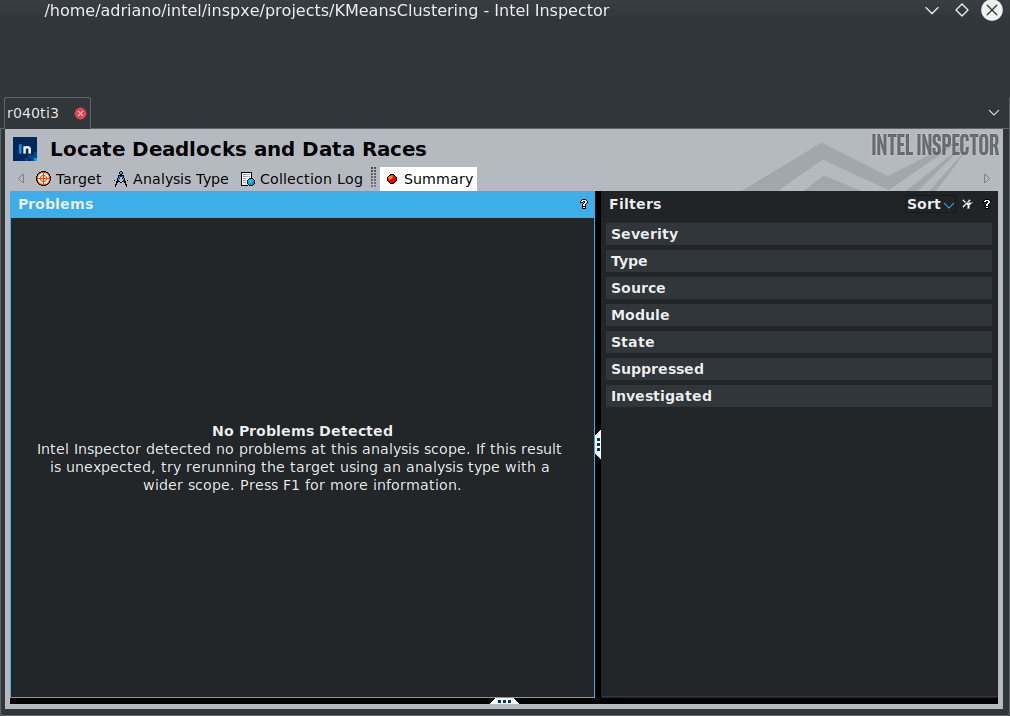
\includegraphics[width=0.5\textwidth]{OpenMP_Inspector}
\caption{Intel Inspector}
\end{figure}
as it can be seen in the above image.\\
OpenMP code was also profiled using Intel's Vtune Profiler that showed optimal core usage when trying to run the last test case
(50000 points and 512 clusters):\\
\begin{figure}[H]
\centering
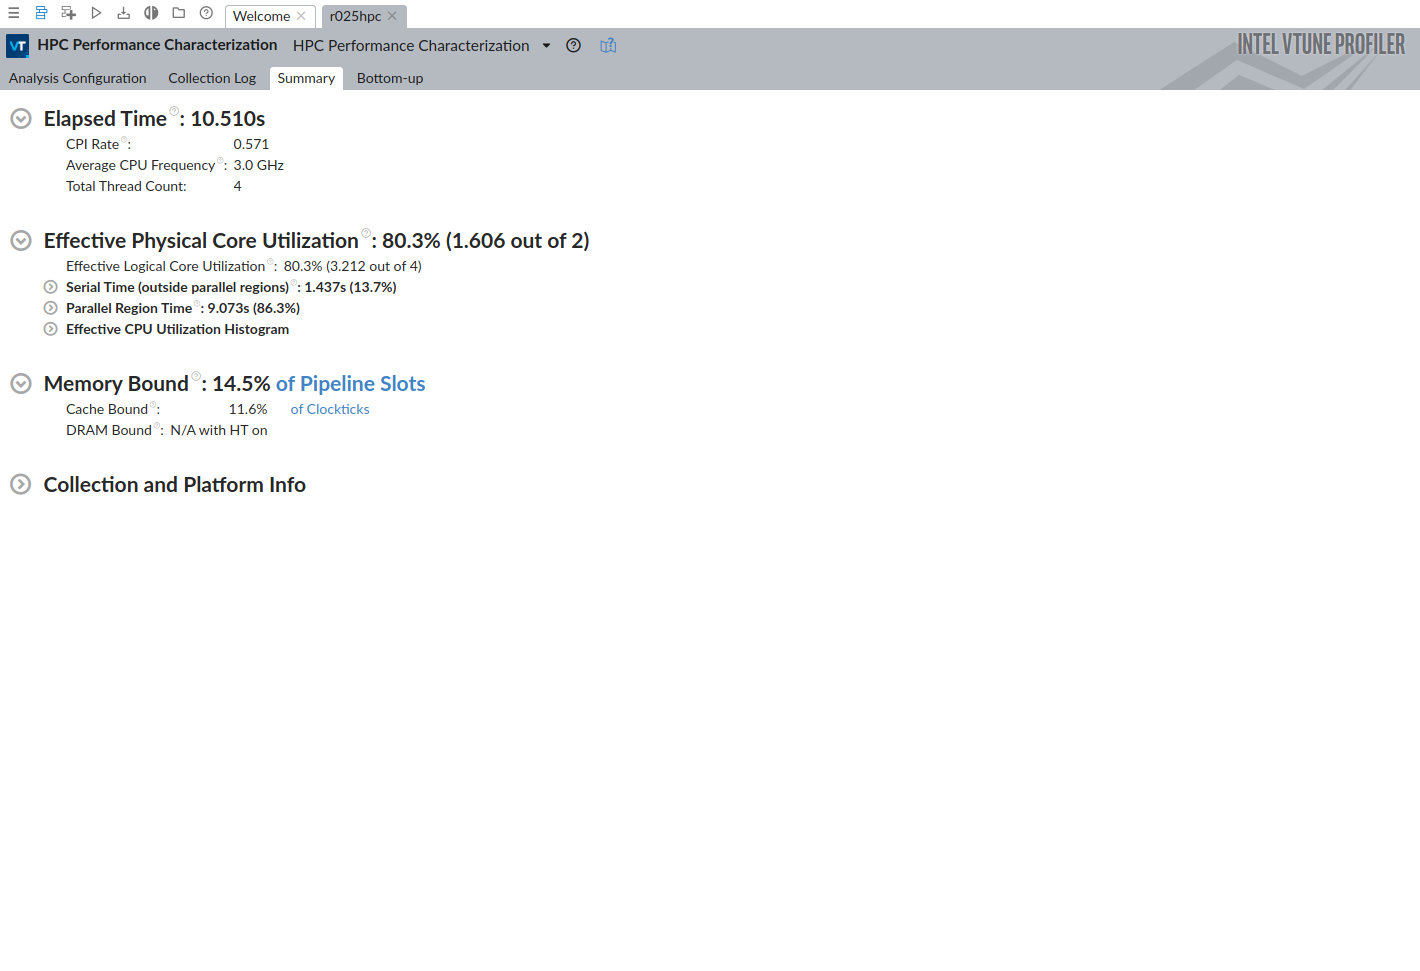
\includegraphics[width=0.5\textwidth]{OpenMP_Vtune_Profiler}
\caption{Intel Vtune Profiler}
\end{figure}
Finally, the CUDA version was profiled using NVidia's profiler called nvprof:\\
\begin{figure}[H]
\centering
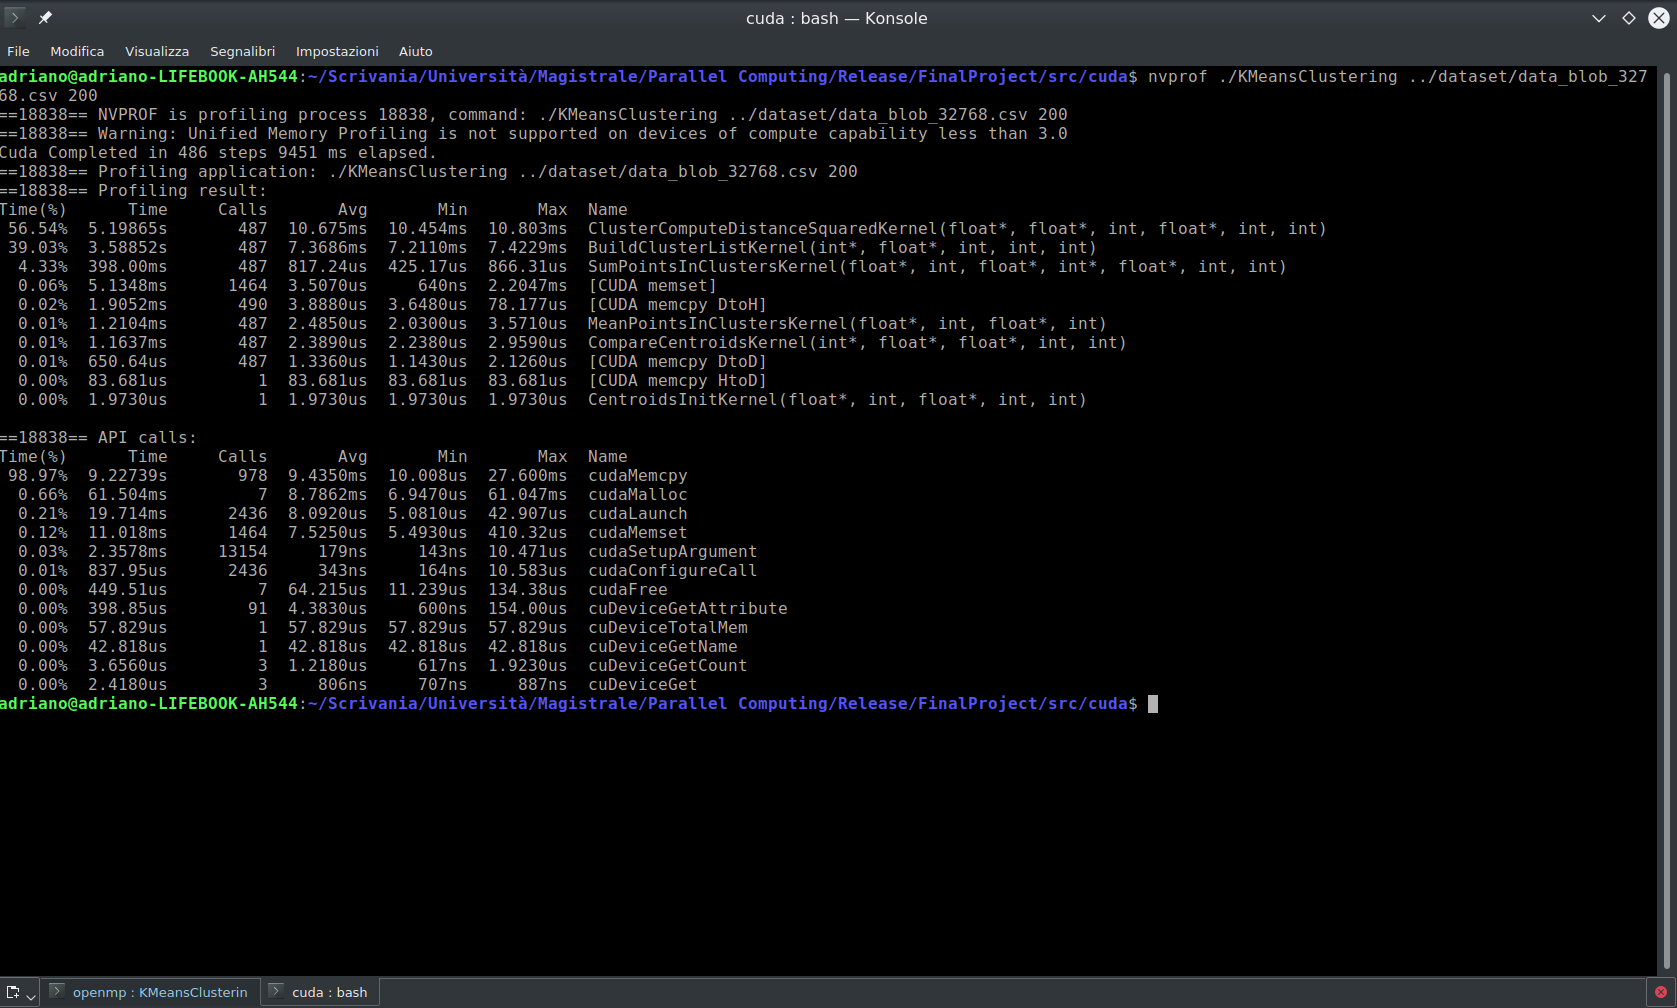
\includegraphics[width=0.5\textwidth]{Cuda_NVProf}
\caption{NVidia NVProf}
\end{figure}
that, as it can be seen from the above image, highlights the top kernels that required most of the time.\\
In particular the kernels `ClusterComputeDistanceSquaredKernel' and `BuildClusterListKernel' are slower than the others.\\
These two function are slower since they need to calculate and then find the nearest centroid for each point in the dataset.\\
This means that the time required to perform these two calculations will grow linearly as the number of points or centroids 
increases.
\end{document}
